% ---------------------------------------------------------------------------
%  Suggestion: place in Section 3, beside Table 1 (the six groups of children
%  of card 727), with \ref{fig:topcard} in the paragraph before it.
%  Generated from the certificate by gen_tikz.py; edit that, not this.
% ---------------------------------------------------------------------------
\begin{figure}[H]
\centering
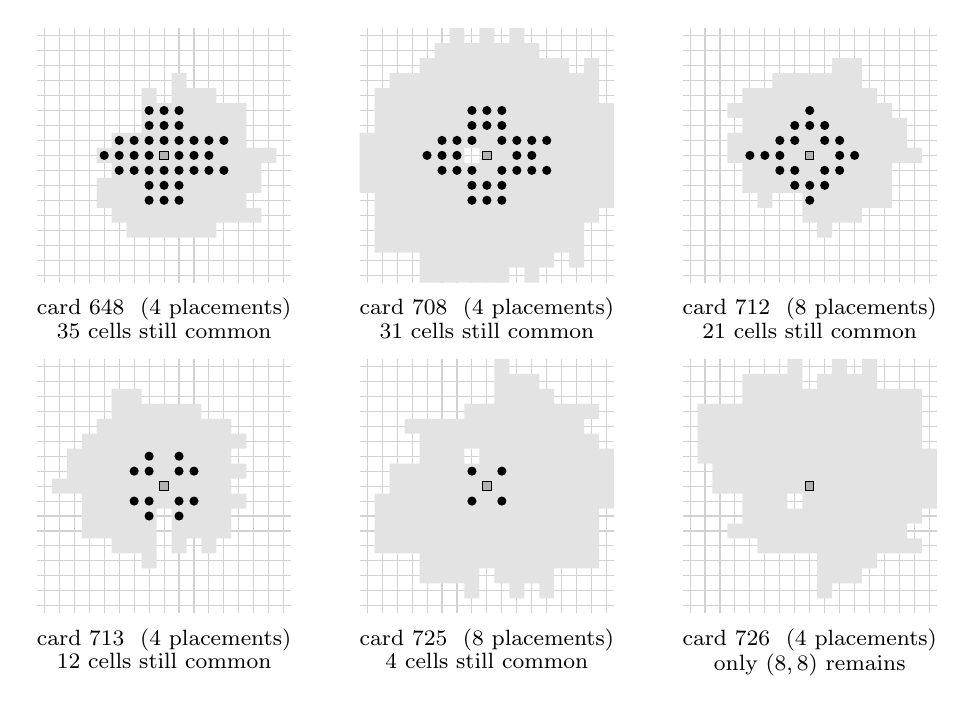
\begin{tikzpicture}[x=1.9mm,y=1.9mm,font=\small]
\begin{scope}[xshift=0.0cm,yshift=0.0cm]
\draw[gray!35,step=1] (-.5,-.5) grid (16.5,16.5);
\fill[gray!22] \foreach \x/\y in {6/3,7/3,8/3,9/3,10/3,11/3,5/4,6/4,7/4,8/4,9/4,10/4,11/4,12/4,13/4,14/4,4/5,5/5,6/5,7/5,8/5,9/5,10/5,11/5,12/5,13/5,4/6,5/6,6/6,7/6,8/6,9/6,10/6,11/6,12/6,13/6,14/6,5/7,6/7,7/7,8/7,9/7,10/7,11/7,12/7,13/7,14/7,4/8,5/8,6/8,7/8,8/8,9/8,10/8,11/8,12/8,13/8,14/8,15/8,5/9,6/9,7/9,8/9,9/9,10/9,11/9,12/9,13/9,7/10,8/10,9/10,10/10,11/10,12/10,13/10,7/11,8/11,9/11,10/11,11/11,12/11,13/11,7/12,9/12,10/12,11/12,9/13}{(\x-.5,\y-.5) rectangle (\x+.5,\y+.5)};
\fill \foreach \x/\y in {7/5,8/5,9/5,7/6,8/6,9/6,5/7,6/7,7/7,8/7,9/7,10/7,11/7,12/7,4/8,5/8,6/8,7/8,9/8,10/8,11/8,5/9,6/9,7/9,8/9,9/9,10/9,11/9,12/9,7/10,8/10,9/10,7/11,8/11,9/11}{(\x,\y) circle (.58mm)};
\filldraw[fill=gray!60] (7.72,7.72) rectangle (8.28,8.28);
\node[below,font=\footnotesize] at (8,-.9) {card 648 \ (4 placements)};
\node[below,font=\footnotesize,yshift=-3.1mm] at (8,-.9) {$35$ cells still common};
\end{scope}
\begin{scope}[xshift=4.1cm,yshift=0.0cm]
\draw[gray!35,step=1] (-.5,-.5) grid (16.5,16.5);
\fill[gray!22] \foreach \x/\y in {4/0,5/0,6/0,7/0,8/0,9/0,11/0,4/1,5/1,6/1,7/1,8/1,9/1,10/1,11/1,12/1,14/1,1/2,2/2,3/2,4/2,5/2,6/2,7/2,8/2,9/2,10/2,11/2,12/2,13/2,14/2,1/3,2/3,3/3,4/3,5/3,6/3,7/3,8/3,9/3,10/3,11/3,12/3,13/3,14/3,1/4,2/4,3/4,4/4,5/4,6/4,7/4,8/4,9/4,10/4,11/4,12/4,13/4,14/4,15/4,1/5,2/5,3/5,4/5,5/5,6/5,7/5,8/5,9/5,10/5,11/5,12/5,13/5,14/5,15/5,16/5,0/6,1/6,2/6,3/6,4/6,5/6,6/6,7/6,8/6,9/6,10/6,11/6,12/6,13/6,14/6,15/6,16/6,0/7,1/7,2/7,3/7,4/7,5/7,6/7,7/7,8/7,9/7,10/7,11/7,12/7,13/7,14/7,15/7,16/7,0/8,1/8,2/8,3/8,4/8,5/8,6/8,8/8,9/8,10/8,11/8,12/8,13/8,14/8,15/8,16/8,0/9,1/9,2/9,3/9,4/9,5/9,6/9,7/9,8/9,9/9,10/9,11/9,12/9,13/9,14/9,15/9,16/9,1/10,2/10,3/10,4/10,5/10,6/10,7/10,8/10,9/10,10/10,11/10,12/10,13/10,14/10,15/10,16/10,1/11,2/11,3/11,4/11,5/11,6/11,7/11,8/11,9/11,10/11,11/11,12/11,13/11,14/11,15/11,16/11,1/12,2/12,3/12,4/12,5/12,6/12,7/12,8/12,9/12,10/12,11/12,12/12,13/12,14/12,15/12,2/13,3/13,4/13,5/13,6/13,7/13,8/13,9/13,10/13,11/13,12/13,13/13,14/13,15/13,4/14,5/14,6/14,7/14,8/14,9/14,10/14,11/14,12/14,13/14,15/14,5/15,6/15,7/15,8/15,9/15,10/15,11/15,6/16,8/16,10/16}{(\x-.5,\y-.5) rectangle (\x+.5,\y+.5)};
\fill \foreach \x/\y in {7/5,8/5,9/5,7/6,8/6,9/6,5/7,6/7,7/7,9/7,10/7,11/7,12/7,4/8,5/8,6/8,10/8,11/8,5/9,6/9,7/9,9/9,10/9,11/9,12/9,7/10,8/10,9/10,7/11,8/11,9/11}{(\x,\y) circle (.58mm)};
\filldraw[fill=gray!60] (7.72,7.72) rectangle (8.28,8.28);
\node[below,font=\footnotesize] at (8,-.9) {card 708 \ (4 placements)};
\node[below,font=\footnotesize,yshift=-3.1mm] at (8,-.9) {$31$ cells still common};
\end{scope}
\begin{scope}[xshift=8.2cm,yshift=0.0cm]
\draw[gray!35,step=1] (-.5,-.5) grid (16.5,16.5);
\fill[gray!22] \foreach \x/\y in {9/3,8/4,9/4,10/4,11/4,5/5,8/5,9/5,10/5,11/5,12/5,13/5,4/6,5/6,6/6,7/6,8/6,9/6,10/6,11/6,12/6,13/6,4/7,5/7,6/7,7/7,8/7,9/7,10/7,11/7,12/7,13/7,3/8,4/8,5/8,6/8,7/8,8/8,9/8,10/8,11/8,12/8,13/8,14/8,15/8,3/9,4/9,5/9,6/9,7/9,8/9,9/9,10/9,11/9,12/9,13/9,14/9,4/10,5/10,6/10,7/10,8/10,9/10,10/10,11/10,12/10,13/10,14/10,3/11,4/11,5/11,6/11,7/11,8/11,9/11,10/11,11/11,12/11,13/11,4/12,5/12,6/12,7/12,8/12,9/12,10/12,11/12,12/12,6/13,7/13,8/13,9/13,10/13,11/13,10/14,11/14}{(\x-.5,\y-.5) rectangle (\x+.5,\y+.5)};
\fill \foreach \x/\y in {8/5,7/6,8/6,9/6,6/7,7/7,9/7,10/7,4/8,5/8,6/8,10/8,11/8,6/9,7/9,9/9,10/9,7/10,8/10,9/10,8/11}{(\x,\y) circle (.58mm)};
\filldraw[fill=gray!60] (7.72,7.72) rectangle (8.28,8.28);
\node[below,font=\footnotesize] at (8,-.9) {card 712 \ (8 placements)};
\node[below,font=\footnotesize,yshift=-3.1mm] at (8,-.9) {$21$ cells still common};
\end{scope}
\begin{scope}[xshift=0.0cm,yshift=-4.2cm]
\draw[gray!35,step=1] (-.5,-.5) grid (16.5,16.5);
\fill[gray!22] \foreach \x/\y in {7/3,5/4,6/4,7/4,9/4,11/4,3/5,4/5,5/5,6/5,7/5,9/5,10/5,11/5,12/5,3/6,4/6,5/6,6/6,7/6,9/6,10/6,11/6,12/6,3/7,4/7,5/7,6/7,7/7,8/7,9/7,10/7,11/7,12/7,13/7,1/8,2/8,3/8,4/8,5/8,6/8,7/8,8/8,9/8,10/8,11/8,12/8,2/9,3/9,4/9,5/9,6/9,7/9,8/9,9/9,10/9,11/9,12/9,13/9,2/10,3/10,4/10,5/10,6/10,7/10,8/10,9/10,10/10,11/10,12/10,3/11,4/11,5/11,6/11,7/11,8/11,9/11,10/11,11/11,12/11,13/11,4/12,5/12,6/12,7/12,8/12,9/12,10/12,11/12,12/12,5/13,6/13,7/13,8/13,9/13,10/13,5/14,6/14}{(\x-.5,\y-.5) rectangle (\x+.5,\y+.5)};
\fill \foreach \x/\y in {7/6,9/6,6/7,7/7,9/7,10/7,6/9,7/9,9/9,10/9,7/10,9/10}{(\x,\y) circle (.58mm)};
\filldraw[fill=gray!60] (7.72,7.72) rectangle (8.28,8.28);
\node[below,font=\footnotesize] at (8,-.9) {card 713 \ (4 placements)};
\node[below,font=\footnotesize,yshift=-3.1mm] at (8,-.9) {$12$ cells still common};
\end{scope}
\begin{scope}[xshift=4.1cm,yshift=-4.2cm]
\draw[gray!35,step=1] (-.5,-.5) grid (16.5,16.5);
\fill[gray!22] \foreach \x/\y in {7/1,10/1,12/1,4/2,5/2,6/2,7/2,9/2,10/2,11/2,12/2,4/3,5/3,6/3,7/3,8/3,9/3,10/3,11/3,12/3,13/3,14/3,15/3,1/4,2/4,3/4,4/4,5/4,6/4,7/4,8/4,9/4,10/4,11/4,12/4,13/4,14/4,15/4,1/5,2/5,3/5,4/5,5/5,6/5,7/5,8/5,9/5,10/5,11/5,12/5,13/5,14/5,15/5,1/6,2/6,3/6,4/6,5/6,6/6,7/6,8/6,9/6,10/6,11/6,12/6,13/6,14/6,15/6,1/7,2/7,3/7,4/7,5/7,6/7,7/7,8/7,9/7,10/7,11/7,12/7,13/7,14/7,15/7,16/7,2/8,3/8,4/8,5/8,6/8,7/8,8/8,9/8,10/8,11/8,12/8,13/8,14/8,15/8,16/8,2/9,3/9,4/9,5/9,6/9,7/9,8/9,9/9,10/9,11/9,12/9,13/9,14/9,15/9,16/9,4/10,5/10,6/10,8/10,9/10,10/10,11/10,12/10,13/10,14/10,15/10,16/10,4/11,5/11,6/11,7/11,8/11,9/11,10/11,11/11,12/11,13/11,14/11,15/11,3/12,4/12,5/12,6/12,7/12,8/12,9/12,10/12,11/12,12/12,13/12,14/12,7/13,8/13,9/13,10/13,11/13,12/13,13/13,14/13,15/13,9/14,10/14,11/14,12/14,9/15,10/15,11/15,9/16}{(\x-.5,\y-.5) rectangle (\x+.5,\y+.5)};
\fill \foreach \x/\y in {7/7,9/7,7/9,9/9}{(\x,\y) circle (.58mm)};
\filldraw[fill=gray!60] (7.72,7.72) rectangle (8.28,8.28);
\node[below,font=\footnotesize] at (8,-.9) {card 725 \ (8 placements)};
\node[below,font=\footnotesize,yshift=-3.1mm] at (8,-.9) {$4$ cells still common};
\end{scope}
\begin{scope}[xshift=8.2cm,yshift=-4.2cm]
\draw[gray!35,step=1] (-.5,-.5) grid (16.5,16.5);
\fill[gray!22] \foreach \x/\y in {9/1,9/2,10/2,11/2,9/3,10/3,11/3,12/3,5/4,6/4,7/4,8/4,9/4,10/4,11/4,12/4,13/4,14/4,15/4,3/5,4/5,5/5,6/5,7/5,8/5,9/5,10/5,11/5,12/5,13/5,14/5,4/6,5/6,6/6,7/6,8/6,9/6,10/6,11/6,12/6,13/6,14/6,15/6,4/7,5/7,6/7,8/7,9/7,10/7,11/7,12/7,13/7,14/7,15/7,16/7,2/8,3/8,4/8,5/8,6/8,7/8,8/8,9/8,10/8,11/8,12/8,13/8,14/8,15/8,16/8,2/9,3/9,4/9,5/9,6/9,7/9,8/9,9/9,10/9,11/9,12/9,13/9,14/9,15/9,16/9,1/10,2/10,3/10,4/10,5/10,6/10,7/10,8/10,9/10,10/10,11/10,12/10,13/10,14/10,15/10,16/10,1/11,2/11,3/11,4/11,5/11,6/11,7/11,8/11,9/11,10/11,11/11,12/11,13/11,14/11,15/11,1/12,2/12,3/12,4/12,5/12,6/12,7/12,8/12,9/12,10/12,11/12,12/12,13/12,14/12,15/12,1/13,2/13,3/13,4/13,5/13,6/13,7/13,8/13,9/13,10/13,11/13,12/13,13/13,14/13,15/13,4/14,5/14,6/14,7/14,8/14,9/14,10/14,11/14,12/14,13/14,14/14,15/14,4/15,5/15,6/15,7/15,9/15,10/15,11/15,12/15,7/16,10/16,12/16}{(\x-.5,\y-.5) rectangle (\x+.5,\y+.5)};
% no cell other than $(8,8)$ is still common
\filldraw[fill=gray!60] (7.72,7.72) rectangle (8.28,8.28);
\node[below,font=\footnotesize] at (8,-.9) {card 726 \ (4 placements)};
\node[below,font=\footnotesize,yshift=-3.1mm] at (8,-.9) {only $(8,8)$ remains};
\end{scope}
\end{tikzpicture}
\caption{The $32$ children of card $727$, grouped by the card they come from;
the card number and the number of its placements are printed below each panel.
Light cells are one placed envelope of the group. The black dots are the cells
still common to every envelope listed up to and including that group, apart from
the pivot $(8,8)$ itself, which is drawn as a grey square throughout: $35,31,21,
12,4$ and finally $0$ of them. So the intersection of all $32$ envelopes is
exactly $\{(8,8)\}$, and Maker's claim there leaves nothing to require ---
$A_{727}=\varnothing$.}
\label{fig:topcard}
\end{figure}
